\documentclass[sigconf]{acmart}

\usepackage{booktabs} % For formal tables


% Copyright
%\setcopyright{none}
%\setcopyright{acmcopyright}
%\setcopyright{acmlicensed}
\setcopyright{rightsretained}
%\setcopyright{usgov}
%\setcopyright{usgovmixed}
%\setcopyright{cagov}
%\setcopyright{cagovmixed}


% DOI
\acmDOI{10.475/123_4}

% ISBN
\acmISBN{123-4567-24-567/08/06}

%Conference
\acmConference[WOODSTOCK'97]{ACM Woodstock conference}{July 1997}{El
  Paso, Texas USA} 
\acmYear{1997}
\copyrightyear{2016}

\acmPrice{15.00}


\begin{document}
\title{SIG Proceedings Paper in LaTeX Format}
\titlenote{Produces the permission block, and
  copyright information}
\subtitle{Extended Abstract}
\subtitlenote{The full version of the author's guide is available as
  \texttt{acmart.pdf} document}


\author{Ben Trovato}
\authornote{Dr.~Trovato insisted his name be first.}
\orcid{1234-5678-9012}
\affiliation{%
  \institution{Institute for Clarity in Documentation}
  \streetaddress{P.O. Box 1212}
  \city{Dublin} 
  \state{Ohio} 
  \postcode{43017-6221}
}
\email{trovato@corporation.com}

\author{G.K.M. Tobin}
\authornote{The secretary disavows any knowledge of this author's actions.}
\affiliation{%
  \institution{Institute for Clarity in Documentation}
  \streetaddress{P.O. Box 1212}
  \city{Dublin} 
  \state{Ohio} 
  \postcode{43017-6221}
}
\email{webmaster@marysville-ohio.com}

\author{Lars Th{\o}rv{\"a}ld}
\authornote{This author is the
  one who did all the really hard work.}
\affiliation{%
  \institution{The Th{\o}rv{\"a}ld Group}
  \streetaddress{1 Th{\o}rv{\"a}ld Circle}
  \city{Hekla} 
  \country{Iceland}}
\email{larst@affiliation.org}

\author{Lawrence P. Leipuner}
\affiliation{
  \institution{Brookhaven Laboratories}
  \streetaddress{P.O. Box 5000}}
\email{lleipuner@researchlabs.org}

\author{Sean Fogarty}
\affiliation{%
  \institution{NASA Ames Research Center}
  \city{Moffett Field}
  \state{California} 
  \postcode{94035}}
\email{fogartys@amesres.org}

\author{Charles Palmer}
\affiliation{%
  \institution{Palmer Research Laboratories}
  \streetaddress{8600 Datapoint Drive}
  \city{San Antonio}
  \state{Texas} 
  \postcode{78229}}
\email{cpalmer@prl.com}

\author{John Smith}
\affiliation{\institution{The Th{\o}rv{\"a}ld Group}}
\email{jsmith@affiliation.org}

\author{Julius P.~Kumquat}
\affiliation{\institution{The Kumquat Consortium}}
\email{jpkumquat@consortium.net}

% The default list of authors is too long for headers}
\renewcommand{\shortauthors}{B. Trovato et al.}


\begin{abstract}
This paper provides a sample of a \LaTeX\ document which conforms,
somewhat loosely, to the formatting guidelines for
ACM SIG Proceedings\footnote{This is an abstract footnote}. 
\end{abstract}

%
% The code below should be generated by the tool at
% http://dl.acm.org/ccs.cfm
% Please copy and paste the code instead of the example below. 
%
\begin{CCSXML}
<ccs2012>
 <concept>
  <concept_id>10010520.10010553.10010562</concept_id>
  <concept_desc>Computer systems organization~Embedded systems</concept_desc>
  <concept_significance>500</concept_significance>
 </concept>
 <concept>
  <concept_id>10010520.10010575.10010755</concept_id>
  <concept_desc>Computer systems organization~Redundancy</concept_desc>
  <concept_significance>300</concept_significance>
 </concept>
 <concept>
  <concept_id>10010520.10010553.10010554</concept_id>
  <concept_desc>Computer systems organization~Robotics</concept_desc>
  <concept_significance>100</concept_significance>
 </concept>
 <concept>
  <concept_id>10003033.10003083.10003095</concept_id>
  <concept_desc>Networks~Network reliability</concept_desc>
  <concept_significance>100</concept_significance>
 </concept>
</ccs2012>  
\end{CCSXML}

\ccsdesc[500]{Computer systems organization~Embedded systems}
\ccsdesc[300]{Computer systems organization~Redundancy}
\ccsdesc{Computer systems organization~Robotics}
\ccsdesc[100]{Networks~Network reliability}

% We no longer use \terms command
%\terms{Theory}

\keywords{ACM proceedings, \LaTeX, text tagging}


\maketitle

\section{Introduction}

 
Vindinium is a popular online AI competition which has attracted many players and developers to work out the best strategy to gather gold while avoiding getting killed. In these attempts, many AI techniques has been applied, such as minimax, Breadth-First Search(BFS), Monte-Carlo Tree Search(MCTS) etc. But limitation exists because of too much possibilities and problems such as the prisoners dilemma. Some strategies play tricks and seek opportunity in irregular ways. Most solutions rely on fine design and rational consideration.
Some strategies based on reinforcement learning have achieved much success in artificial intelligence competitions. In this article, we try to use techniques of reinforcement learning to solve the problem.
 

\section{The Body of The Paper}
This section discussed important agent considerations. Our implementation and our results.

\subsection{Agent Environment}


P.E.A.S.\\\\
Performance:\\
Resources (Mines owned)\\
  Environment:\\
Two dimensional grid environment\\
  Multiple competing agents:\\
Actuators:\\
  Four directions of movement and remaining still\\
Sensors:\\
  Fully observable environment\\\\
  
Environment Properties\\
  
Fully observable environment: Vindinium agents perceive all possible information about their environment \\

Deterministic: Knowledge of previous states and the current state and action performed can be used to determine the next series of states. \\
  
Sequential:Vindinium has a limited amount of turns that it plays out in.The finite amount of turns and Knowledge of previous states and current states can be used to predict future states.\\


Dynamic: All agents only have five possible actions each turn i.e. to travel east, west, north, south or to stay still. Also the changes to the grid environment itself are merely boolean operational changes in states.\\

Multi-agent: Vindinium at its core is about competing with other agents for resources\\

\subsection{Agent Architecture}
According to the result of  P.E.A.S, the better choice of the agent architecture is reinforcement learning. In reinforcement learning, the ultimate goal of the agent is to attain the maximum reward in total and in each of step, the agent could get a single special reward from the environment.  

In Vindinium, the agent could get the whole environment information by sensors in every time step, like the current position of agents, the position of the obstacle and so on. That means the state of the agent that succeeds in retaining all relevant information. In other words, the environment has the Markov property. If an environment has the Markov property, then the next state could be predicted and the expected reward was given to the current state and action in one-step dynamics. By iterating, one can predict all the future states and expected rewards from the knowledge only of the current state or the by the experience from the past to current. 

Since the task of Vindinium is satisfied the Markov property, so it is a Markov decision process (MDP). In the world of Vindinium, the state and action spaces of the agent are finite.  Agents' actions are limited, they can only do four actions: "go north", "go south", "go west" and "go east".  Besides, the environment is also limited, the agent could receive the limited state of the environment in every single step, like the map of Vindinium. So, the problem of Vindinium could be defined as a finite Markov decision process (finite MDP).

To compute the optimal policies for Vindinium, the dynamic programming (DP) is a better choice even though the classical DP algorithms' utility are limited in reinforcement learning. In this case, we use policy iteration to compute the optimal policies.

For the policy iteration which is used in Vindinium, an initial value is given at the stage of beginning. The next stage is the policy evaluation. In this stage, calculating the expected value in the probability of taking action a in state s under policy  pi. In iterative policy evaluation, vk+1 from vk and the iteration stop when the quantity max(vk+1 - vk) among in the state s is sufficiently small. The final step is the policy improvement. To find better policies, it is necessary to compute the value function for a policy. By doing this, it could improve the policy that the agent would be used

\subsection{ Specification}
Vindinum is an online and continuous competition and the server can receive, send and process commands of HTTP and JSON format. So, the client can be implemented easily on different platforms. Starter packs of many popular language (such as c, c++, python, etc) are provided on the official website with clients to process the HTTP and JSON parsing work.
 
In our project, we use python (python3) as our development language because its clean and straightforward syntax, powerful libraries and widespread use in the area of artificial intelligence and machine learning. We also choose pycharm as our integrated development environment(IDE) and github as the version management tool.
 
We also used the Pandas Library as our database tool because of its high-performance and easy-to-use data structure for processing and analysis.

\subsection{Implementation}

The entire project was built on the use of advantage learning with purely softmax action selection. 

Advantage Learning is a form of reinforcement learning similar to Q-learning except that uses advantages instead of Q-values. For state x and action u, the advantage for that state action pair A(x,u)  is related to the Q value Q(x,u)
$A(x,u)=max(Q(x,u')) + (Q(x,u) -max(Q(x,u'))) * k/dt$

In terms of implementing this, a lookup table combined with an update functions were used. There are two functions that update the probability of choosing an action based on the performance measure of mines owned in the case they have either a negative or positive change. 

Each contributing previous state is update with a reward or punishment based on its contribution to gaining or losing mines. The negative function decreases the state's probability as seen below.

In the case of vindinium the action selection was simplified given the time frame. States were reduced to abstractions in order to increase the ability to learn in a short amount of time. example Health =low, medium or high

Softmax action selection:\\
next to best action selection,facilitates learning for the agent with reasonable level of exploration.
 


 
Shortest Path Planning\\

As shown in Figure 2, obstacles which cannot be passed are represented with negative number. The hero’ s position is represented with 0 which means the step to reach is 0. Positive number represents the shortest steps to go to the locate. see Figure 3.

In terms of creating, modifying and updating the backend of the reinforcement learning agent, the pandas software library was used. It is used mostly for data manipulation and analysis, thus very appropriate for managing the reinforcement agents backend and analysis of its performance.



\begin{figure}
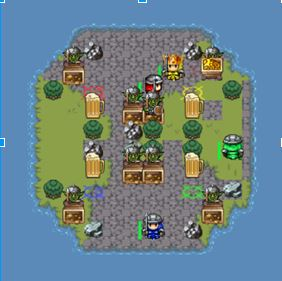
\includegraphics[height=1in, width=1in]{move1.jpg}
\caption{map representation}
\end{figure}

\begin{figure}
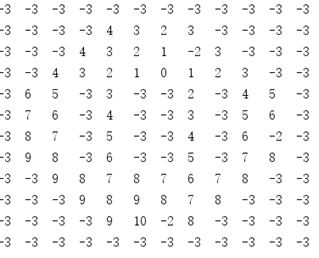
\includegraphics[height=1in, width=1in]{move2.jpg}
\caption{map representation}
\end{figure}

\subsection{Results}
After training over 80 games,we gained 4110 entries in the database. In the 100 entries with the highest decision weight (weight>=0.852539), there are 9 of attacking and 91 of going mine. This indicates the hero has learned from the experience that taking control of mines can earn reward as well as killing others. While in the 100 entries with lowest weight (weight<=0.400055), there are 40 of attacking, 9 of going mine and 51 of going pub. Worth to mention that all 40 entries of attacking is under the low health state which means the hero learns to be less aggressive when the HP is low and avoids to be killed.

As shown in Table 1, we do a further statistical analysis over all the data and extract the average weights of each decision under different healthy level. It can be viewed that going to take control of mines is the decision of biggest possibility in all cases. While the possibility of going to pub to recover is slightly higher in low HP than medium HP and high HP. This is a good sign but the learning rate is not very ideal. This may because there is more disturbance during the process of learning to go pub. Specifically, when the hero is in low HP and decide to go to the pub, he may be attacked to die by other heroes. And the death will make the hero believe going pub is a wrong decision at that state and give a negative reflection.

We finally increase the winning percentage from 30\% to 70\% by reinforcement learning.

\begin{table*}
 \caption{Actions weighting after learning}
 \label{tab:commands}
 \begin{tabular}{cccl}
   \toprule
   	  & Attack & GoMine &  GoPub\\
   \midrule
   High & 0.509118(28.62\%) & 0.764765(43\%)& 0.504718(28.38\%)\\
   Medium & 0.522177(28.82\%) & 0.769719(42.5\%)&
   0.519672(28.68\%)\\
   Low &0.522307(29.18\%) & 0.751547(41.99\%) & 0.516056(28.83\%)\\
   \bottomrule
 \end{tabular}
\end{table*}




\section{Conclusions}
We discuss the P.E.A.S of Vindinium and analyse the agent architecture.  The problem of Vindinium is defined as a finite Markov decision process, using reinforcement learning is a better way to solve the problem. In the stage of the implement, we use policy iteration which is a classical dynamic programming algorithm to compute the optimal policy for the agent. The policy which is used for the agent is under the probability and the expected value. The agent could choose different policy according to the external environment and the information from itself. We achieve a high probability of winning the game by using reinforcement learning by using a small database. By analysing the records in the database of the agent, the average of probability for each policy indicates the agent work nicely and do the right thing with the policy iteration. 

Even the agent's performance is good, but it still has some of part working not well. It still needs to train and let it have a previous knowledge and training cost too much of time. But we believe, by updating the algorithm and using the new method to the agent, it could lead the cost of agent more to decrease and the agent could have a better performance.
%\end{document}  % This is where a 'short' article might terminate



\appendix
%Appendix A
\section{Headings in Appendices}

\subsection{Introduction}
\subsection{The Body of the Paper}
\subsubsection{Agent Environment}
\subsubsection{Agent Architecture}
\subsubsection{Specification}
\subsubsection{Implementation}
\subsubsection{Results}
\subsection{Conclusions}
\subsection{References}



\bibliographystyle{ACM-Reference-Format}
\bibliography{sigproc} 

\end{document}
